%% Creator: Inkscape inkscape 0.92.2, www.inkscape.org
%% PDF/EPS/PS + LaTeX output extension by Johan Engelen, 2010
%% Accompanies image file 'bat12.eps' (pdf, eps, ps)
%%
%% To include the image in your LaTeX document, write
%%   \input{<filename>.pdf_tex}
%%  instead of
%%   \includegraphics{<filename>.pdf}
%% To scale the image, write
%%   \def\svgwidth{<desired width>}
%%   \input{<filename>.pdf_tex}
%%  instead of
%%   \includegraphics[width=<desired width>]{<filename>.pdf}
%%
%% Images with a different path to the parent latex file can
%% be accessed with the `import' package (which may need to be
%% installed) using
%%   \usepackage{import}
%% in the preamble, and then including the image with
%%   \import{<path to file>}{<filename>.pdf_tex}
%% Alternatively, one can specify
%%   \graphicspath{{<path to file>/}}
%% 
%% For more information, please see info/svg-inkscape on CTAN:
%%   http://tug.ctan.org/tex-archive/info/svg-inkscape
%%


\begingroup%
  \makeatletter%
  \providecommand\color[2][]{%
    \errmessage{(Inkscape) Color is used for the text in Inkscape, but the package 'color.sty' is not loaded}%
    \renewcommand\color[2][]{}%
  }%
  \providecommand\transparent[1]{%
    \errmessage{(Inkscape) Transparency is used (non-zero) for the text in Inkscape, but the package 'transparent.sty' is not loaded}%
    \renewcommand\transparent[1]{}%
  }%
  \providecommand\rotatebox[2]{#2}%
  \ifx\svgwidth\undefined%
    \setlength{\unitlength}{432bp}%
    \ifx\svgscale\undefined%
      \relax%
    \else%
      \setlength{\unitlength}{\unitlength * \real{\svgscale}}%
    \fi%
  \else%
    \setlength{\unitlength}{\svgwidth}%
  \fi%
  \global\let\svgwidth\undefined%
  \global\let\svgscale\undefined%
  \makeatother%
  \begin{picture}(1,0.83333333)%
    \put(0,0){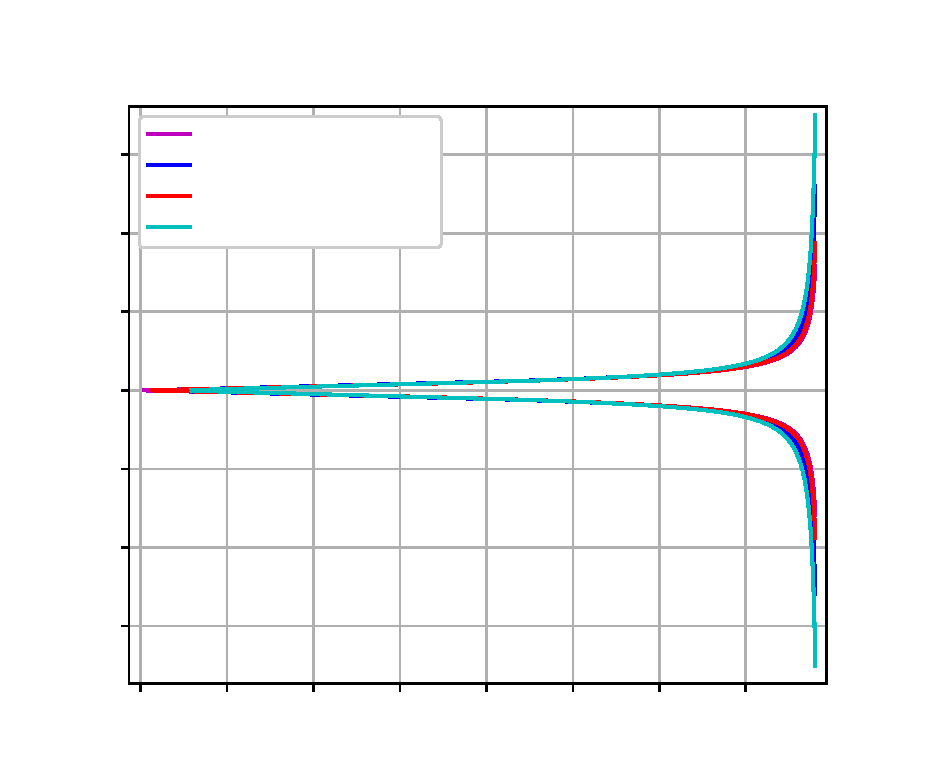
\includegraphics[width=\unitlength]{imagesbat/bat12.eps}}%
    \put(0.11923819,0.05788495){\color[rgb]{0,0,0}\makebox(0,0)[lb]{\smash{0.0}}}%
    \put(0.21531203,0.05788495){\color[rgb]{0,0,0}\makebox(0,0)[lb]{\smash{0.2}}}%
    \put(0.31138425,0.05788495){\color[rgb]{0,0,0}\makebox(0,0)[lb]{\smash{0.4}}}%
    \put(0.40745832,0.05788495){\color[rgb]{0,0,0}\makebox(0,0)[lb]{\smash{0.6}}}%
    \put(0.50353008,0.05788495){\color[rgb]{0,0,0}\makebox(0,0)[lb]{\smash{0.8}}}%
    \put(0.59960415,0.05788495){\color[rgb]{0,0,0}\makebox(0,0)[lb]{\smash{1.0}}}%
    \put(0.69567822,0.05788495){\color[rgb]{0,0,0}\makebox(0,0)[lb]{\smash{1.2}}}%
    \put(0.79174998,0.05788495){\color[rgb]{0,0,0}\makebox(0,0)[lb]{\smash{1.4}}}%
    \put(0.05,0.14706226){\color[rgb]{0,0,0}\makebox(0,0)[lb]{\smash{$-30$}}}%
    \put(0.05,0.23435879){\color[rgb]{0,0,0}\makebox(0,0)[lb]{\smash{$-20$}}}%
    \put(0.05,0.3216574){\color[rgb]{0,0,0}\makebox(0,0)[lb]{\smash{$-10$}}}%
    \put(0.09407546,0.40895601){\color[rgb]{0,0,0}\makebox(0,0)[lb]{\smash{0}}}%
    \put(0.07935486,0.49625462){\color[rgb]{0,0,0}\makebox(0,0)[lb]{\smash{10}}}%
    \put(0.07935486,0.58355323){\color[rgb]{0,0,0}\makebox(0,0)[lb]{\smash{20}}}%
    \put(0.07935486,0.67084952){\color[rgb]{0,0,0}\makebox(0,0)[lb]{\smash{30}}}%
    \put(0.470353008,0.01){\color[rgb]{0,0,0}\makebox(0,0)[lb]{\smash{ $\theta_0 (rad)$}}}%
    \put(0.04524745,0.4){\color[rgb]{0,0,0}\rotatebox{90}{\makebox(0,0)[lb]{\smash{$\hat{\omega_0} $}}}}%
    \put(0.21064814,0.69492128){\color[rgb]{0,0,0}\makebox(0,0)[lb]{\smash{\footnotesize $R=1.0 m, r_2=1.0 cm$}}}%
    \put(0.21064814,0.66030785){\color[rgb]{0,0,0}\makebox(0,0)[lb]{\smash{\footnotesize $R=1.0 m, r_2=5.0 cm$}}}%
    \put(0.21064814,0.62569443){\color[rgb]{0,0,0}\makebox(0,0)[lb]{\smash{\footnotesize $R=0.5 m, r_2=1.0 cm$}}}%
    \put(0.21064814,0.591081){\color[rgb]{0,0,0}\makebox(0,0)[lb]{\smash{\footnotesize $R=0.5 m, r_2=5.0 cm$}}}%
    \put(0.59960415,0.23435879){\color[rgb]{0,0,0}\makebox(0,0)[lb]{\smash{stable}}}%
    \put(0.59960415,0.58355323){\color[rgb]{0,0,0}\makebox(0,0)[lb]{\smash{stable}}}%
    \put(0.75,0.40895601){\color[rgb]{0,0,0}\makebox(0,0)[lb]{\smash{instable}}}%
  \end{picture}%
\endgroup%
